\documentclass[]{report}
\usepackage{graphicx}

% Title Page
\title{{\Huge \emph{myTaxiService}}\linebreak Requirements Analysis and Specification Document}
\author{Belluschi Marco, Cerri Stefano, Di Febbo Francesco}

\begin{document}
\maketitle
\tableofcontents

%INTRODUCTION
\chapter{Introduction}

\section{Purpose}
This document represent the Requirement Analysis and Specification Document (RASD). The main goal of this document is to completely describe the system in terms of functional and non-functional requirements, analyse the real need of the customer to modelling the system, show the constraints and the limit of the software and simulate the typical use cases that will occur after the development. This document is intended to all developer and programmer who have to implement the requirements, to system analyst who want to integrate other system with this one, and could be used as a contractual basis between the customer and the developer.


\section{Scope}
The system described in this document is a taxi service for a large city.
The main goals of the system are: 1) simplify the access of passengers to the service 2) guarantee a fair management of taxi queues.
The system is composed by a web application, a mobile application and a web server.

There are three types of actors that can use the system: visitors, taxi drivers and passengers.
Visitors have only two operations allowed: log in or sign in.
Passengers can use both the web application and the mobile application to request a taxi.
Taxi drivers use only the mobile application to:
\begin{itemize}
	\item confirm to the system that they are going to take care of a certain request from a certain passenger
	\item say if they have finished a ride 
	\item say if they want to finish their workshift.
\end{itemize}

The system, when a passenger request a taxi, informs an available taxi driver (FIFO mode) about the current position of that passenger. 
At this time the taxi driver has two options:
\begin{itemize}
\item accept : the system sends a notification to the passenger with the estimated waiting time
\item reject : the system searches for another available taxi driver
\end{itemize}

The system allows also a passenger to:
\begin{itemize}
\item reserve a taxi by specifying the origin and the destination of the ride
\item share a taxi with others, if possible. In this case the system defines the cost of the ride for each passenger
\end{itemize}

Besides the specific user interfaces for passengers and taxi drivers, the system offers also APIs to enable the development of additional services on top of the basic one.

%\section{Goals}
%\input{introduction/goals.tex}

\section{Definitions, Acronyms, Abbreviations}
\paragraph{Definitions}
\begin{itemize}
	\item User: person that uses the service applications.
	\item Visitor: user that has not registered nor logged in.
	\item Registered user: user that has registered to the service.
	\item Passenger: passenger registered to the service.
	\item Taxi driver: taxi driver registered to the service.
	\item System: the union of software and hardware to be developed and implemented.
	
	
\end{itemize}
\paragraph{Acronyms}
\paragraph{Abbreviations}

\section{Actors}
There are three types of actors that use MyTaxiService:
\begin{itemize}
	\item visitors: they can only log in or sign up
	
	\item passengers: they can request,reserve or share a taxi
	
	\item taxi drivers: they can accept/deny a ride
	
\end{itemize}

\section{Identifying stakeholders}
The main stakeholder of the project is the government of a large city.
The government, with the help of the transport council, decided to improve the actual taxi service with MyTaxiService.
With MyTaxiService the stakeholders want to:

\begin{itemize}
	\item symplify the access of passangers to the service
	\item guarantee a fair management of taxi queues
	\item give the possibility to the passengers to reserve a taxi 
	\item give the possibility to a passenger to share a taxi with other passengers
	
\end{itemize}

\section{Reference documents}
\begin{itemize}
	\item Software Engineering 2 Project AA 2015/2016: Project Description And Rules
	\item Software Engineering 2 Project AA 2015/2016: Assignments 1 and 2 (RASD and DD) 
	
\end{itemize}

\section{Overview}
This document is essentially structured in three parts:
\begin{itemize}
\item Section 1: Introduction: it gives a description of the  document and some basical information about the system. It also identifying the stakeholders and the actors involved.
\item Section 2: Overall Description: it gives general information about the software and hardware product, constraints and assumptions.
\item Section 3: Specific Requirements: this is the core of the document. It describes the functional and non-functional requirements combined with some scenarios. There is also a class diagram that gives an overall representation of the system.
\end{itemize}


%OVERALL DESCRIPTION
\chapter{Overall Description}

\section{Product perspective}
The system is composed by a web application, a mobile application and a web server. The web application runs on most common browsers, namely Chrome, Internet Explorer, Firefox, Safari. It needs a web server that supports PHP. The mobile application needs a platform supporting Android, iOs or Windows Phone. Both applications interact with a DBMS.\newline
Additional functionalities are provided through the use of APIs or interfaces, i.e. taxi reservation and the taxi sharing option.


\section{Product functions}
The system allows different kinds of user to perform different actions. In particular:
\begin{itemize}
  \item Visitors can simply register or log in, thus becoming either a passenger or a taxi driver user.
  \item Passengers can request, reserve and share taxi rides.
  \item Taxi drivers can respond (accept/refuse) to impeding ride requests.
\end{itemize}

\begin{center}
	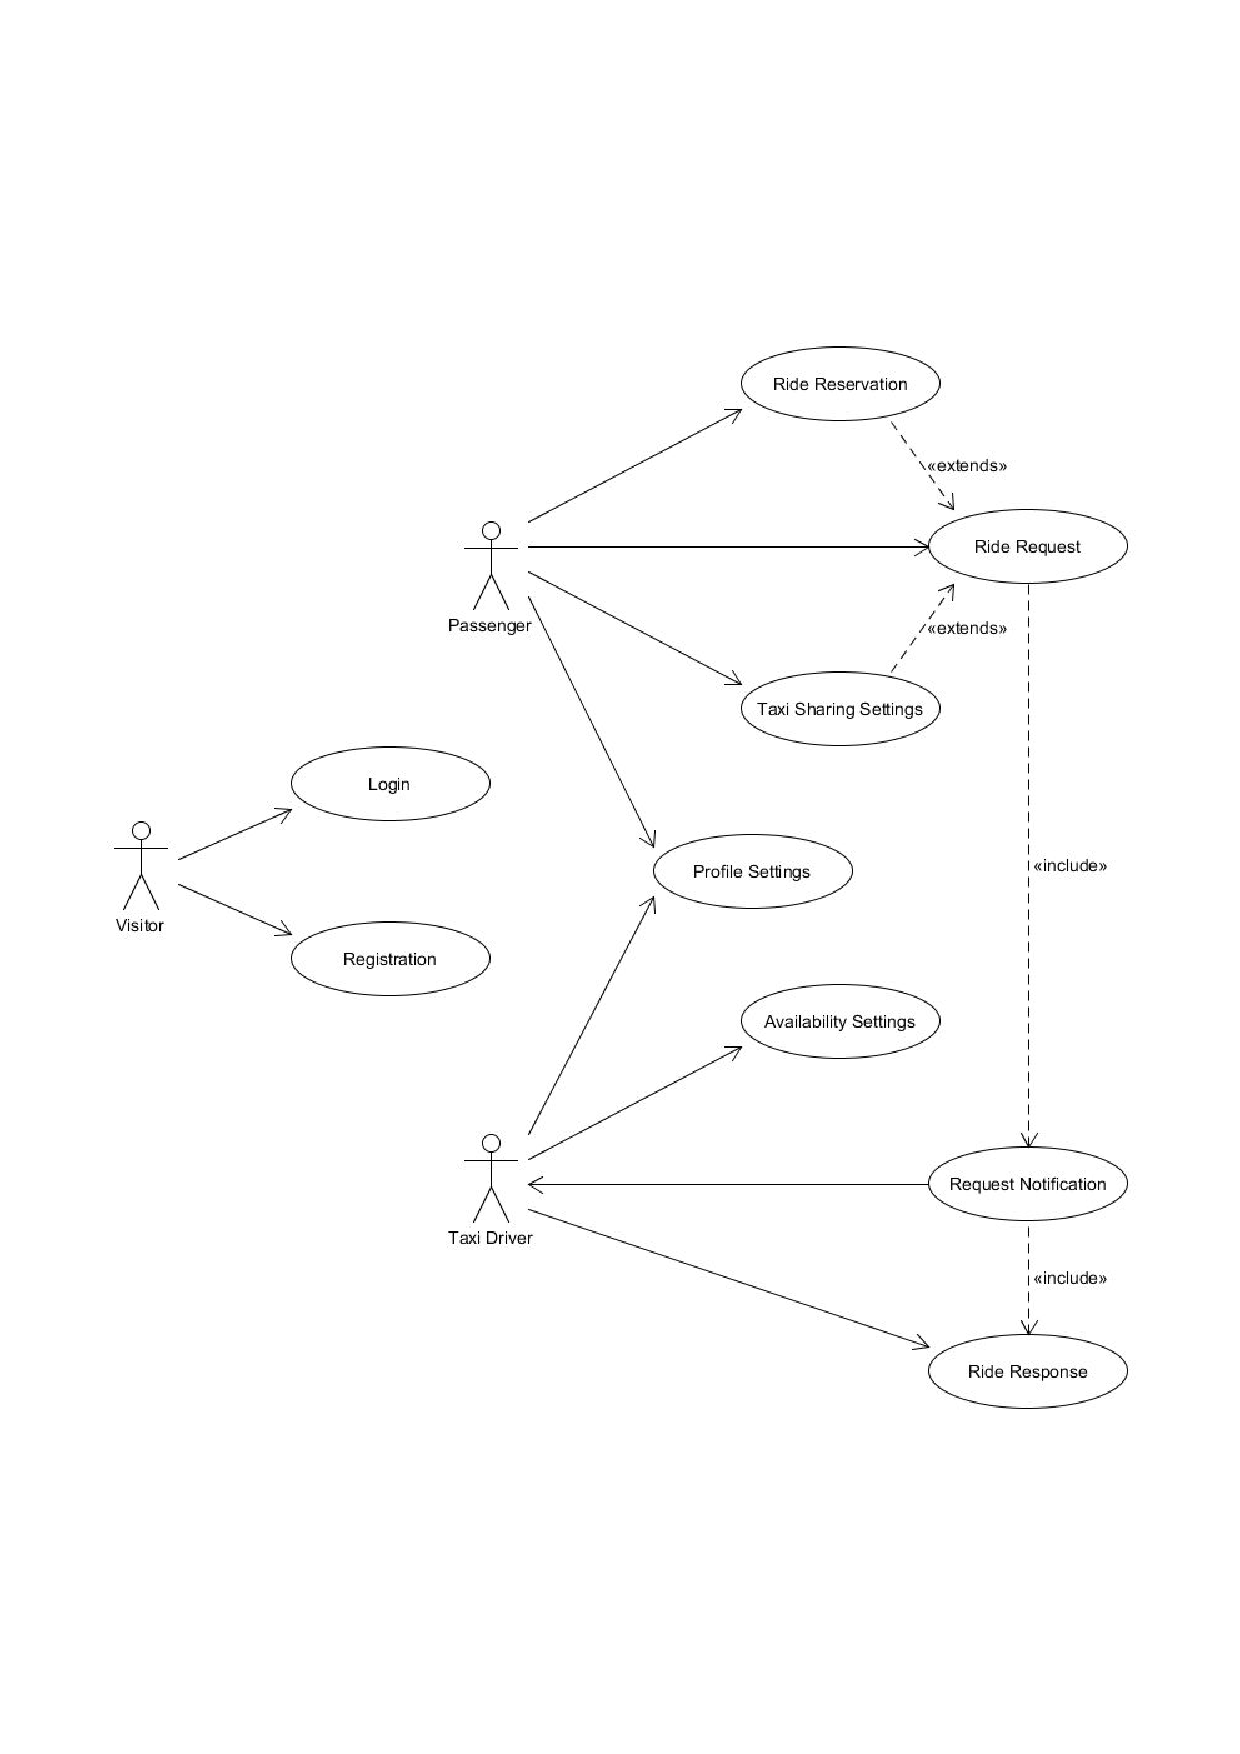
\includegraphics[width=\textwidth]{diagrams/global_use_case}
	{\bf Use case diagram} for {\it myTaxiService}
\end{center}

\begin{center}
	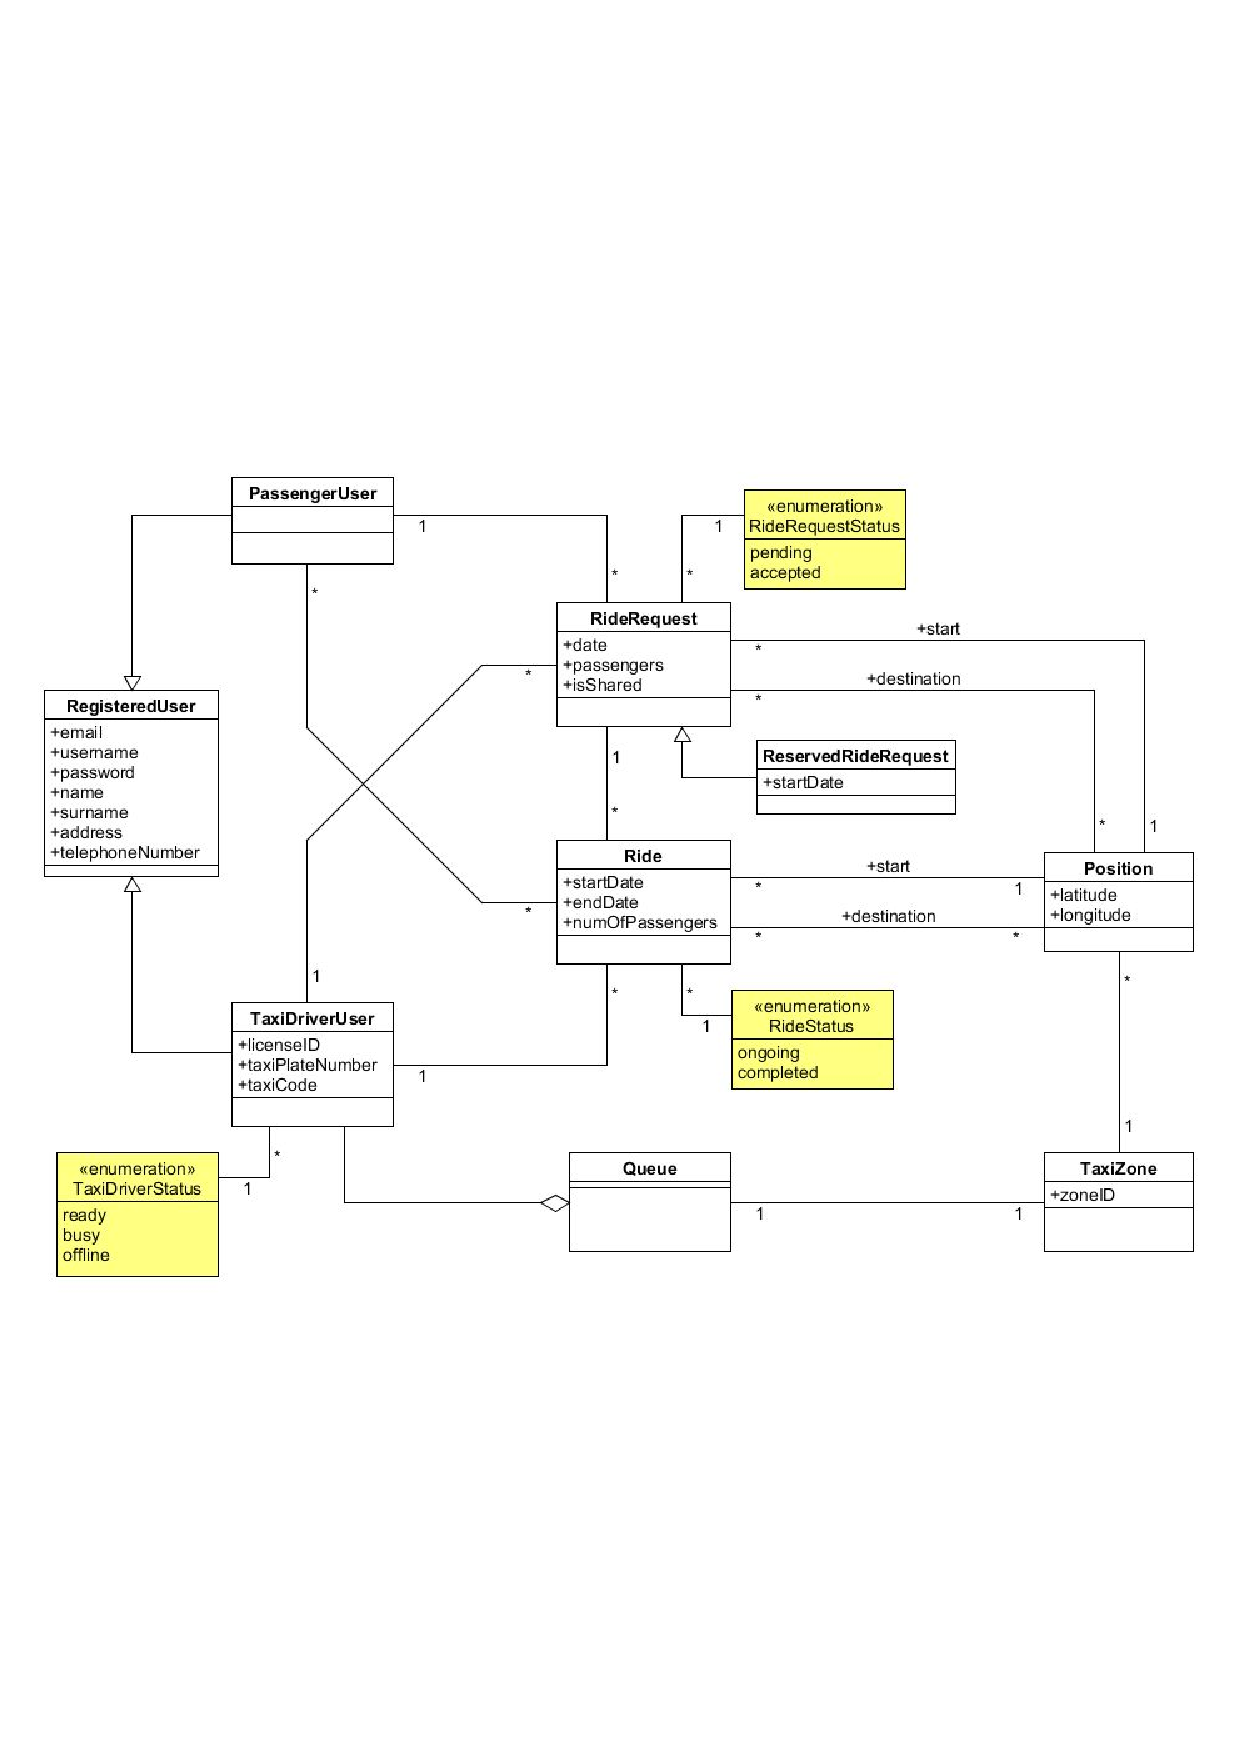
\includegraphics[width=\textwidth]{diagrams/global_class_diagram}
	{\bf Class diagram} for {\it myTaxiService}
\end{center}


\section{User characteristics}
Registered users can be either passengers or taxi drivers.\newline
The system wants to give both an easy way to interact, thus optimizing the taxi service. To do so, passengers must be able to install and use the mobile application, or use the web application. On the contrary, taxi drivers can only install and use the mobile app; besides, their cellphone must be provided with a GPS. All users must have access to the Internet.


\section{Constraints}
\subsection{Regulatory policies}
myTaxiService is a service provided by the public company responsible for public transportation in the city. The user, who reaches this service by web or mobile application, has to agree to License Agreement rather than Privacy policy and Terms of use at registration.\\
The user access and use of the services constitutes his/her agreement to be bound by these Terms, which establishes a contractual relationship between him/her and myTaxiService. If user does not agree to these Terms, he/she may not access or use the services. myTaxiService may immediately terminate these Terms or any services with respect to him/her, or generally cease offering or deny access to the Services or any portion thereof, at any time for any reason.\\
myTaxiService collects the information provided by the user, for example when creating or making changes to services on demand, through contact with customer service or during other communications. This information may include: name, email, phone number, mailing address, profile picture, payment method, products required (for service delivery), delivery receipts and other information user choose to provide. The personal data will be used only to provide the services requested.\\
User is responsible for obtaining the data network access necessary to use the services. User mobile network's data and messaging rates and fees may apply if he/she accesses or uses the services from a wireless-enabled device. User is responsible for acquiring and updating compatible hardware or devices necessary to access and use the service and applications and any updates thereto.\\
myTaxiService does not guarantee that the services, or any portion thereof, will function on any particular hardware or devices. In addition, the services may be subject to malfunctions and delays inherent in the use of the Internet and electronic communications.

\subsection{Hardware limitations}
myTaxiService defines the minimum requirements for using web and mobile applications.
\begin{itemize}
	\item \textit{Web application}\\
	Supported minimum version browsers: Chrome 25, Internet Explorer 10, Firefox 20, Safari 25. Other browsers may also work\\
	Web access at the minimum speed of 1Mbps
	\item \textit{Mobile application}\\
	Operating system: Android, iOS, Windows Phone\\
	Memory: 512MB RAM\\
	Hard drive: 50MB of free space\\
	GPS navigation system (only for taxi drivers)\\
	Web access at the minimum speed of 1Mbps
\end{itemize}

\subsection{Interfaces to other applications}
myTaxiService provides APIs to enable development of additional software on this platform.

\subsection{Parallel operation}
myTaxiService supports parallel operations cause of the nature of service. Many users can access to the service at same time thus system and database have to work with parallel requests.

%\subsection{Audit functions}
%\subsection{Control functions}

\subsection{High-order language requirements}
myTaxiService requires the following high-order languages based on different platforms.
\begin{itemize}
	\item\textit{Web}\\
	HTML 5 and CSS 3 standards.
	\item\textit{Android}\\
	Java 8
	\item\textit{iOS}\\
	Swift 2.0
	\item\textit{Windows Phone}\\
	C\# 6.0
	\item \textit{Server}\\
	MySQL 5.6.19 and PHP 5.6.7
\end{itemize}

%\subsection{Signal handshake protocols}

\subsection{Reliability requirements}
myTaxiService relies on network connections thus reliability issues are equivalent to performance issues.  However, the application should not corrupt server data as a result of its actions. The system has to guarantee whole-time availability.

\subsection{Criticality of the application}
 myTaxiService relies on network systems and servers. Scheduled downtime is acceptable. This system requires a generator backup and redundant power in the event of failover.

\subsection{Safety and security considerations}
myTaxiService guarantees secure communications through AES encryption algorithms.

\section{Assumptions and Dependencies}
\subsection{Assumption}
\begin{itemize}
	\item Passenger requests a ride from web or mobile applications
	\item Passenger sets a correct meeting point
	\item Passenger sets a correct destination
	\item Taxi driver reaches the meeting point
	\item Taxi driver picks up the correct passenger
	\item Accurate taxi driver's locations are known by GPS
	\item Taxi driver reports correctly his availability
	\item The city is divided in taxi zones
	\item The taxi queue in a zone contains only taxi drivers available in that zone
	\item Taxi driver confirms or denies a passenger request call
\end{itemize}

\section{Future implementation}
\begin{itemize}
	\item Every taxi cab will be equipped with automotive navigation system implementing myTaxiService software. Personal phones are not required. This system will improve driving safety providing an easy way of interacting with the application.
	\item myTaxiService will implement an easy-pay system. The system calculates costs according to the route and provides payment methods with credit cards, PayPal, contact-less.
\end{itemize}

%SPECIFIC REQUIREMENTS
\chapter{Specific Requirements}

\section{External Interface Requirements}
\subsection{User interfaces}
The interface of MyTaxiService can be for web application and mobile application. Here will be presented some of the most important pages and screens of MyTaxiService.

\paragraph{Log in:}
	In the figure below is shown MyTaxiService's homepage
	\begin{center}
		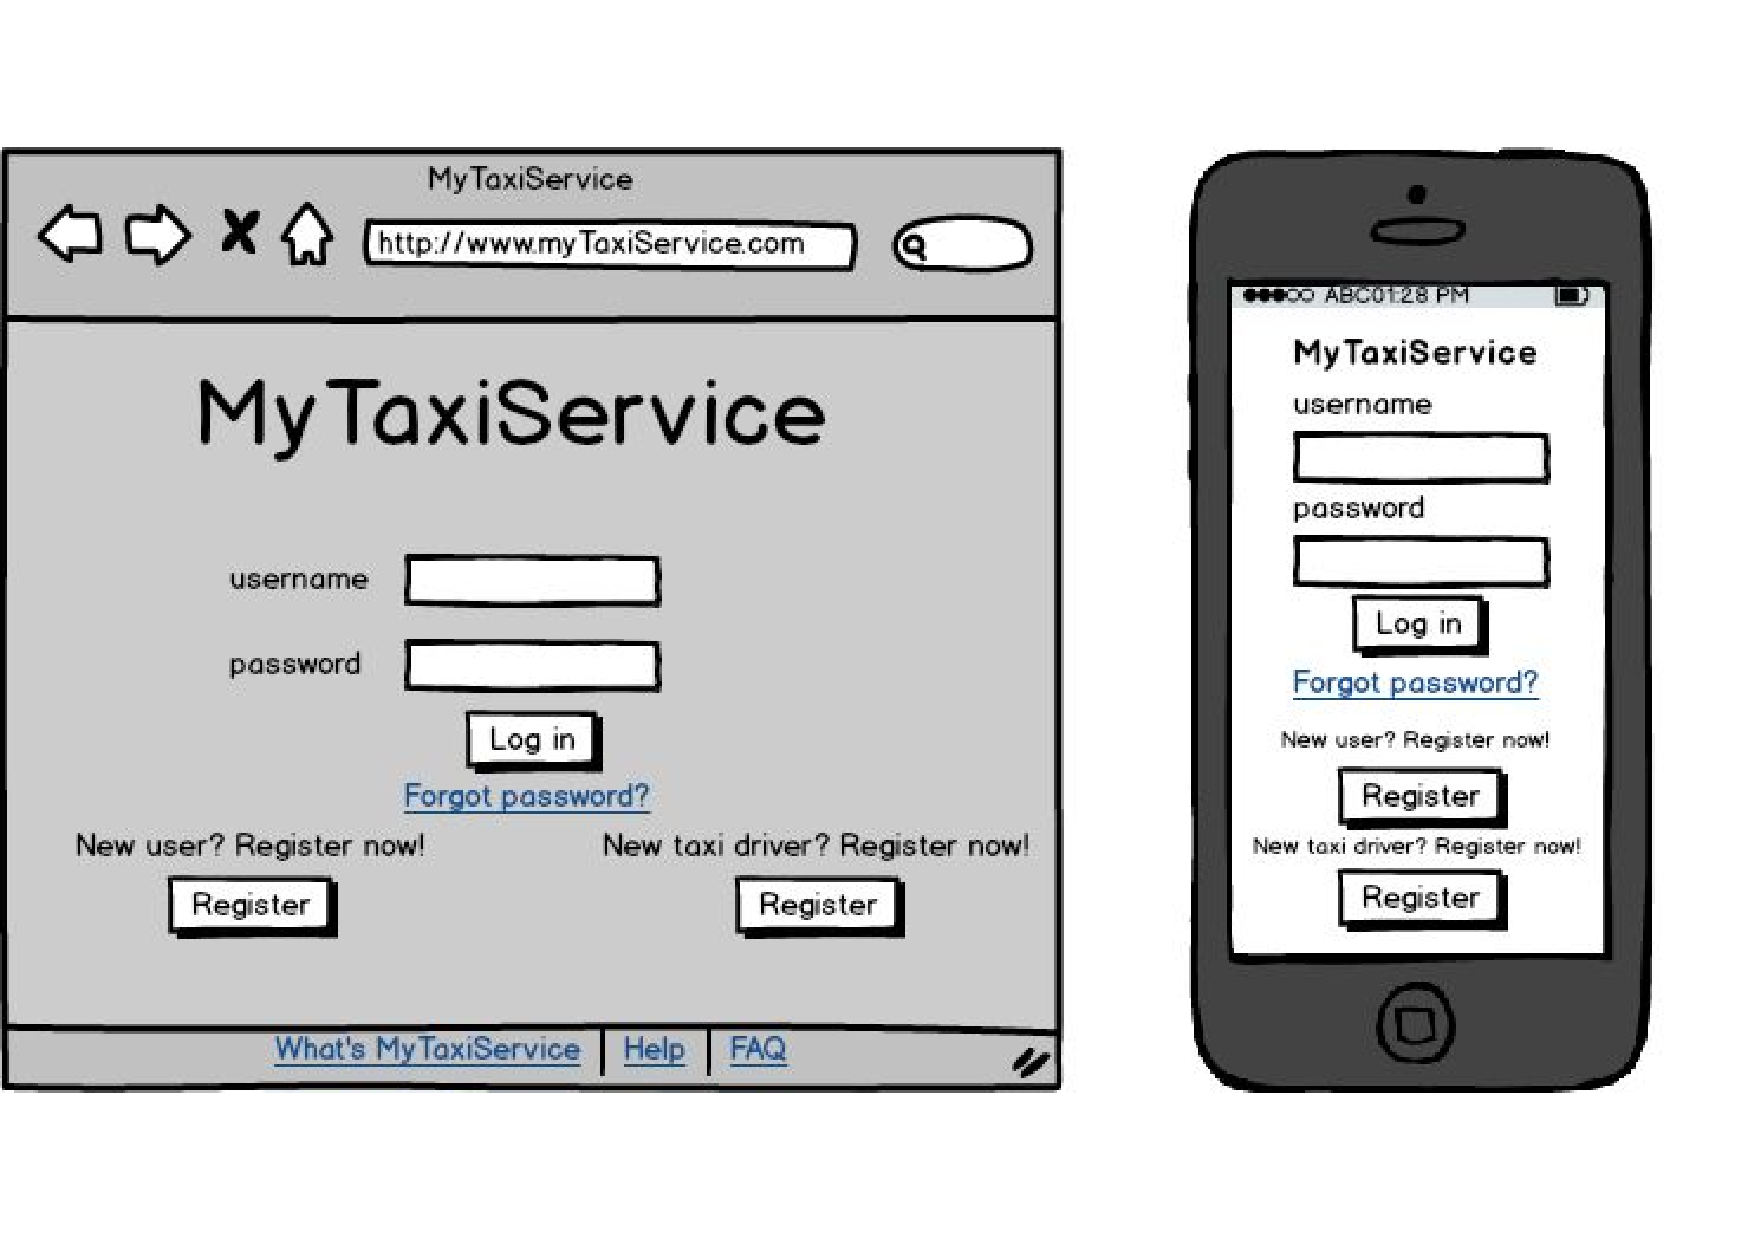
\includegraphics[width=\textwidth]{mockup/login1.pdf}
	\end{center}
	
\paragraph{Registration passenger:}
	View of the visitor that wants to register as a passenger
\begin{center}
	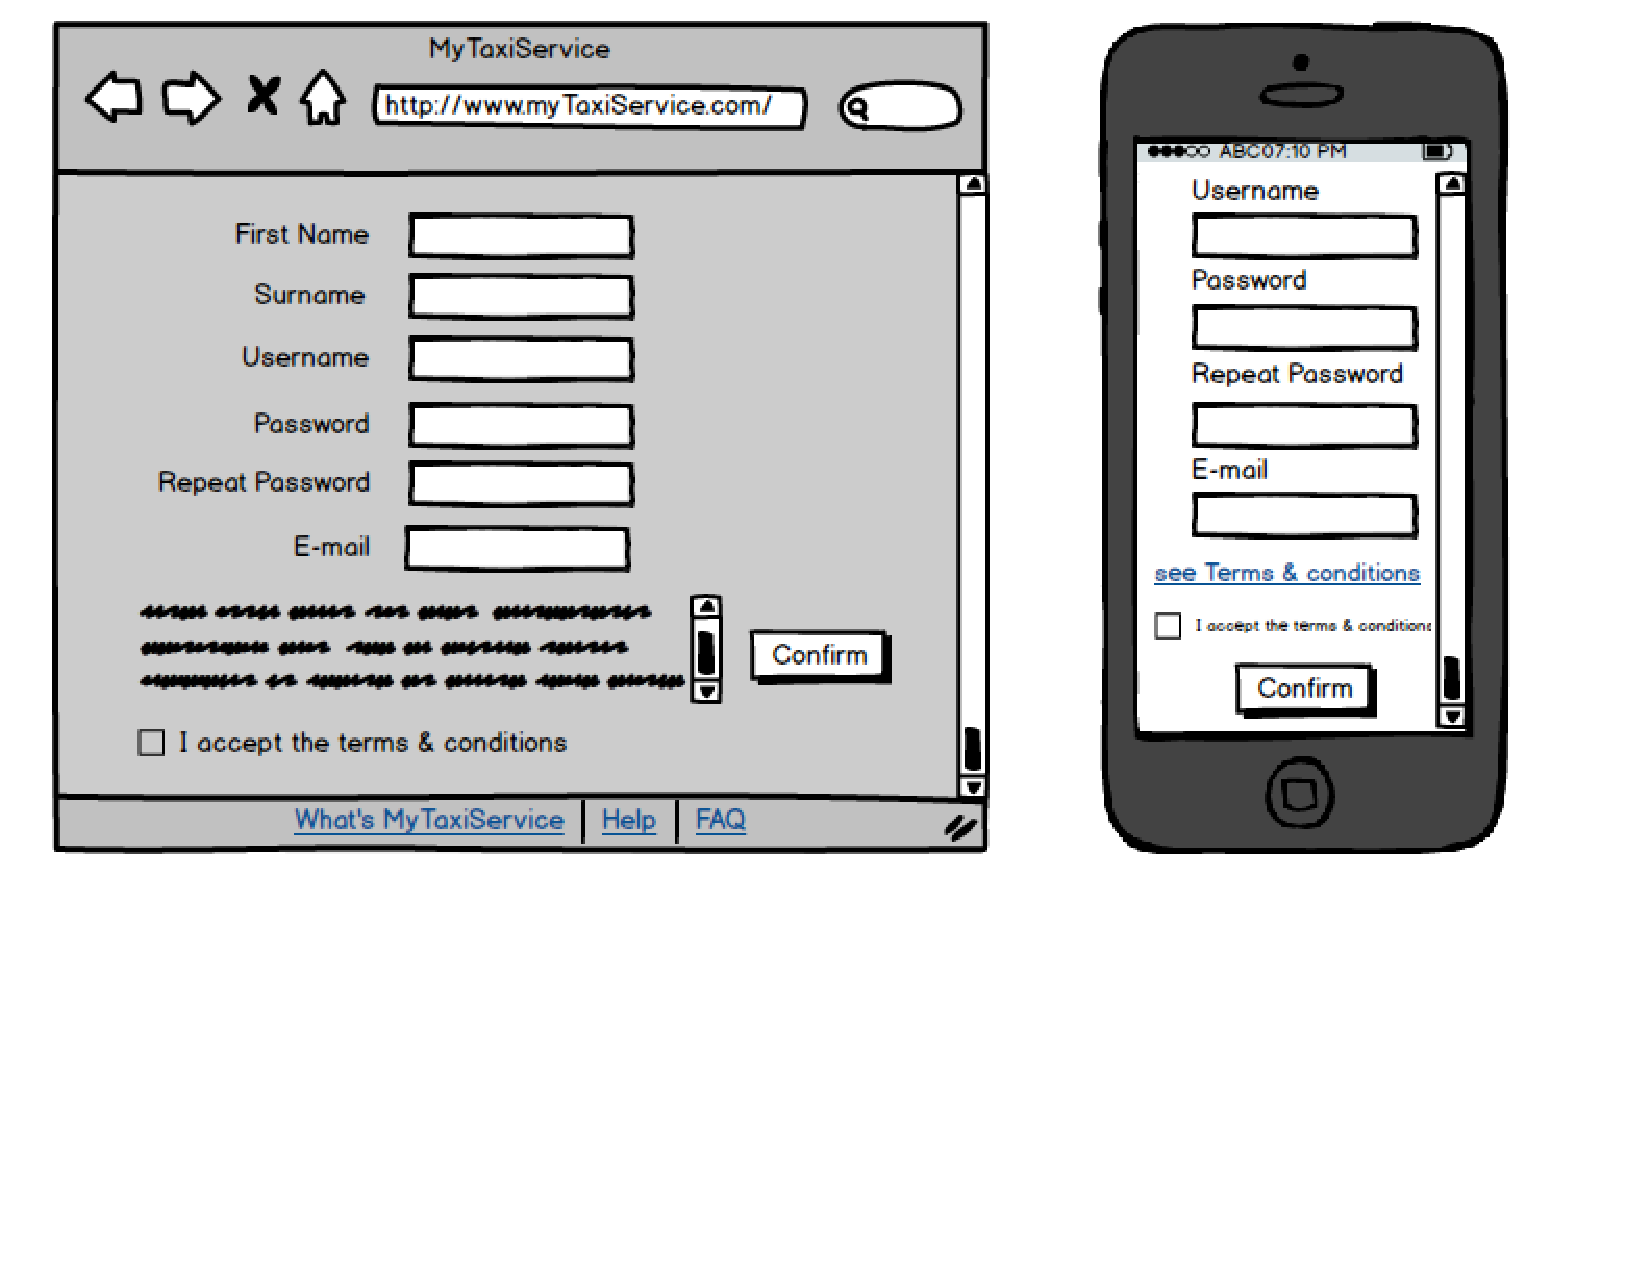
\includegraphics[width=\textwidth]{mockup/registrationPassenger.pdf}
\end{center}
\newpage


\paragraph{Registration taxi Driver:}
	View of the visitor that wants to register as a taxi driver
\begin{center}
	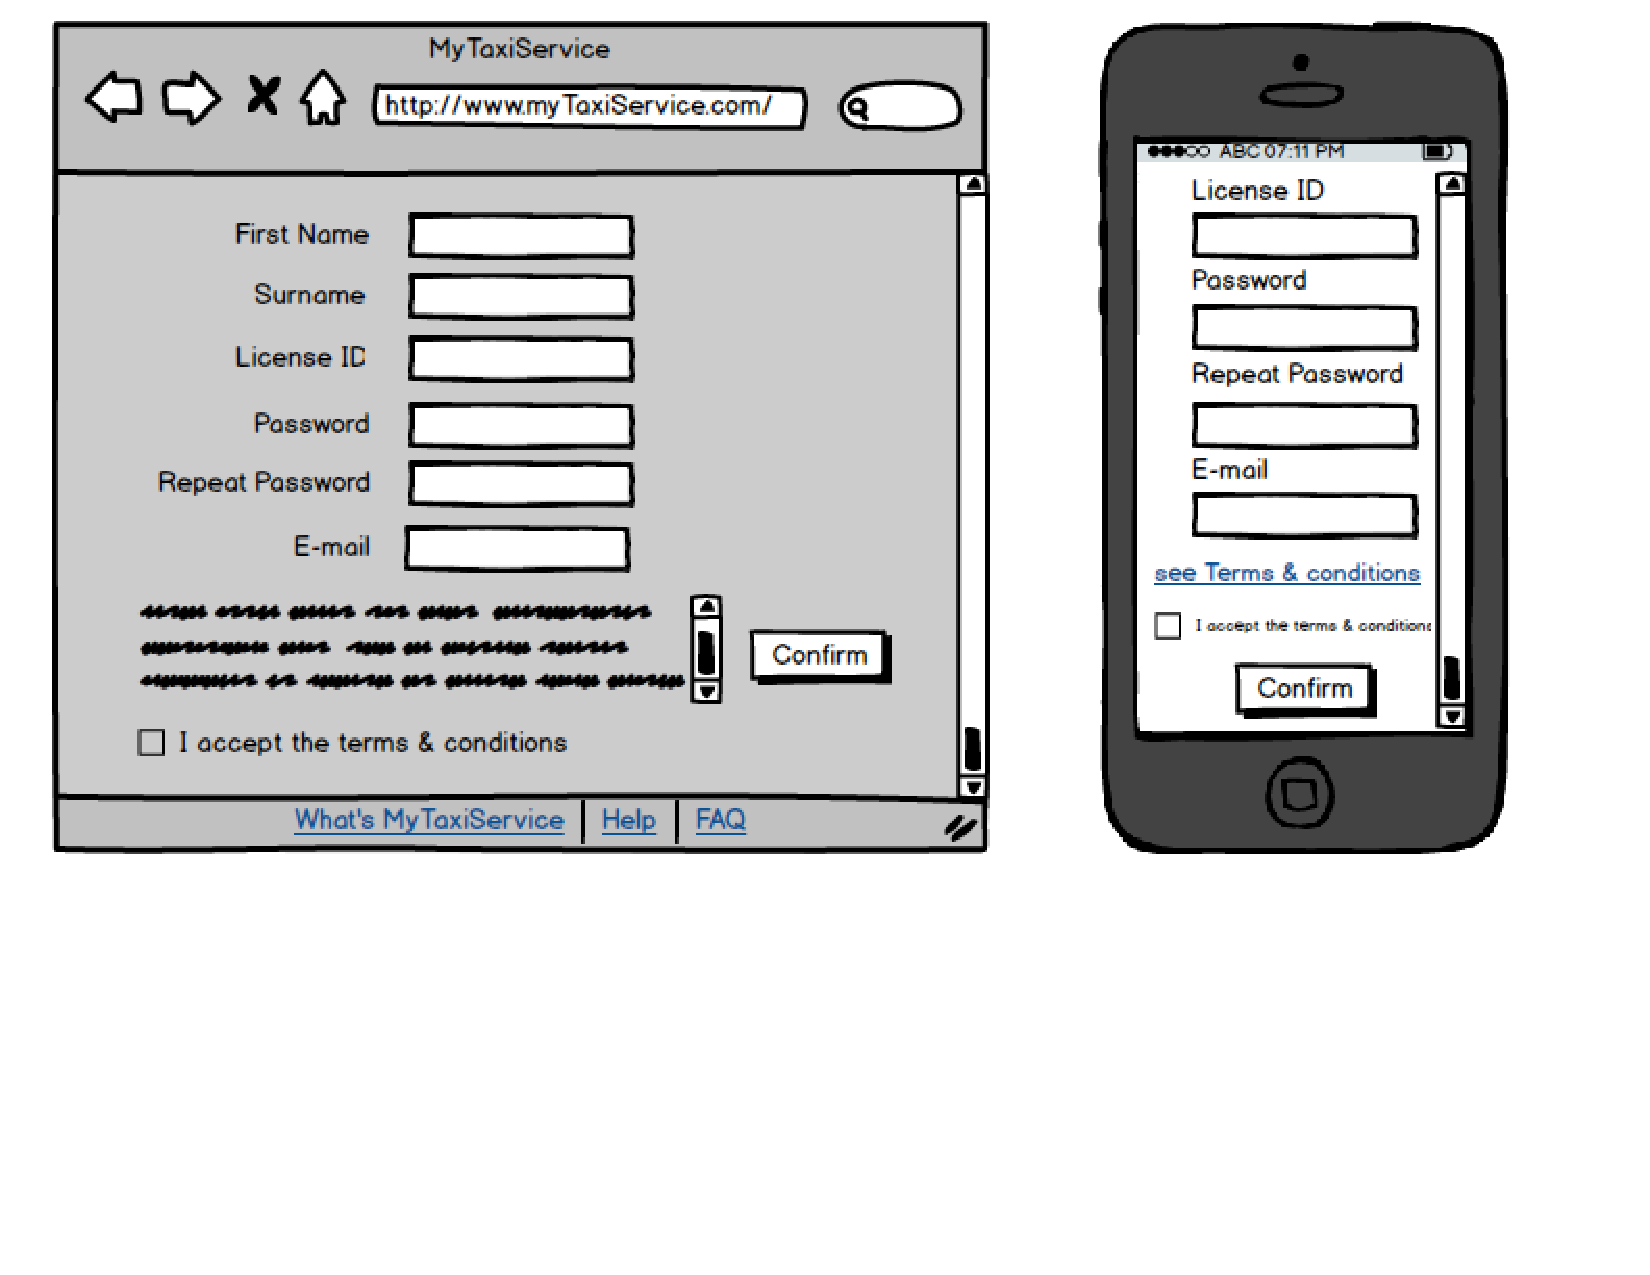
\includegraphics[width=\textwidth]{mockup/registrationTaxiDriver.pdf}
\end{center}
\newpage
\paragraph{Passenger view:}
View of the passenger
\begin{center}
	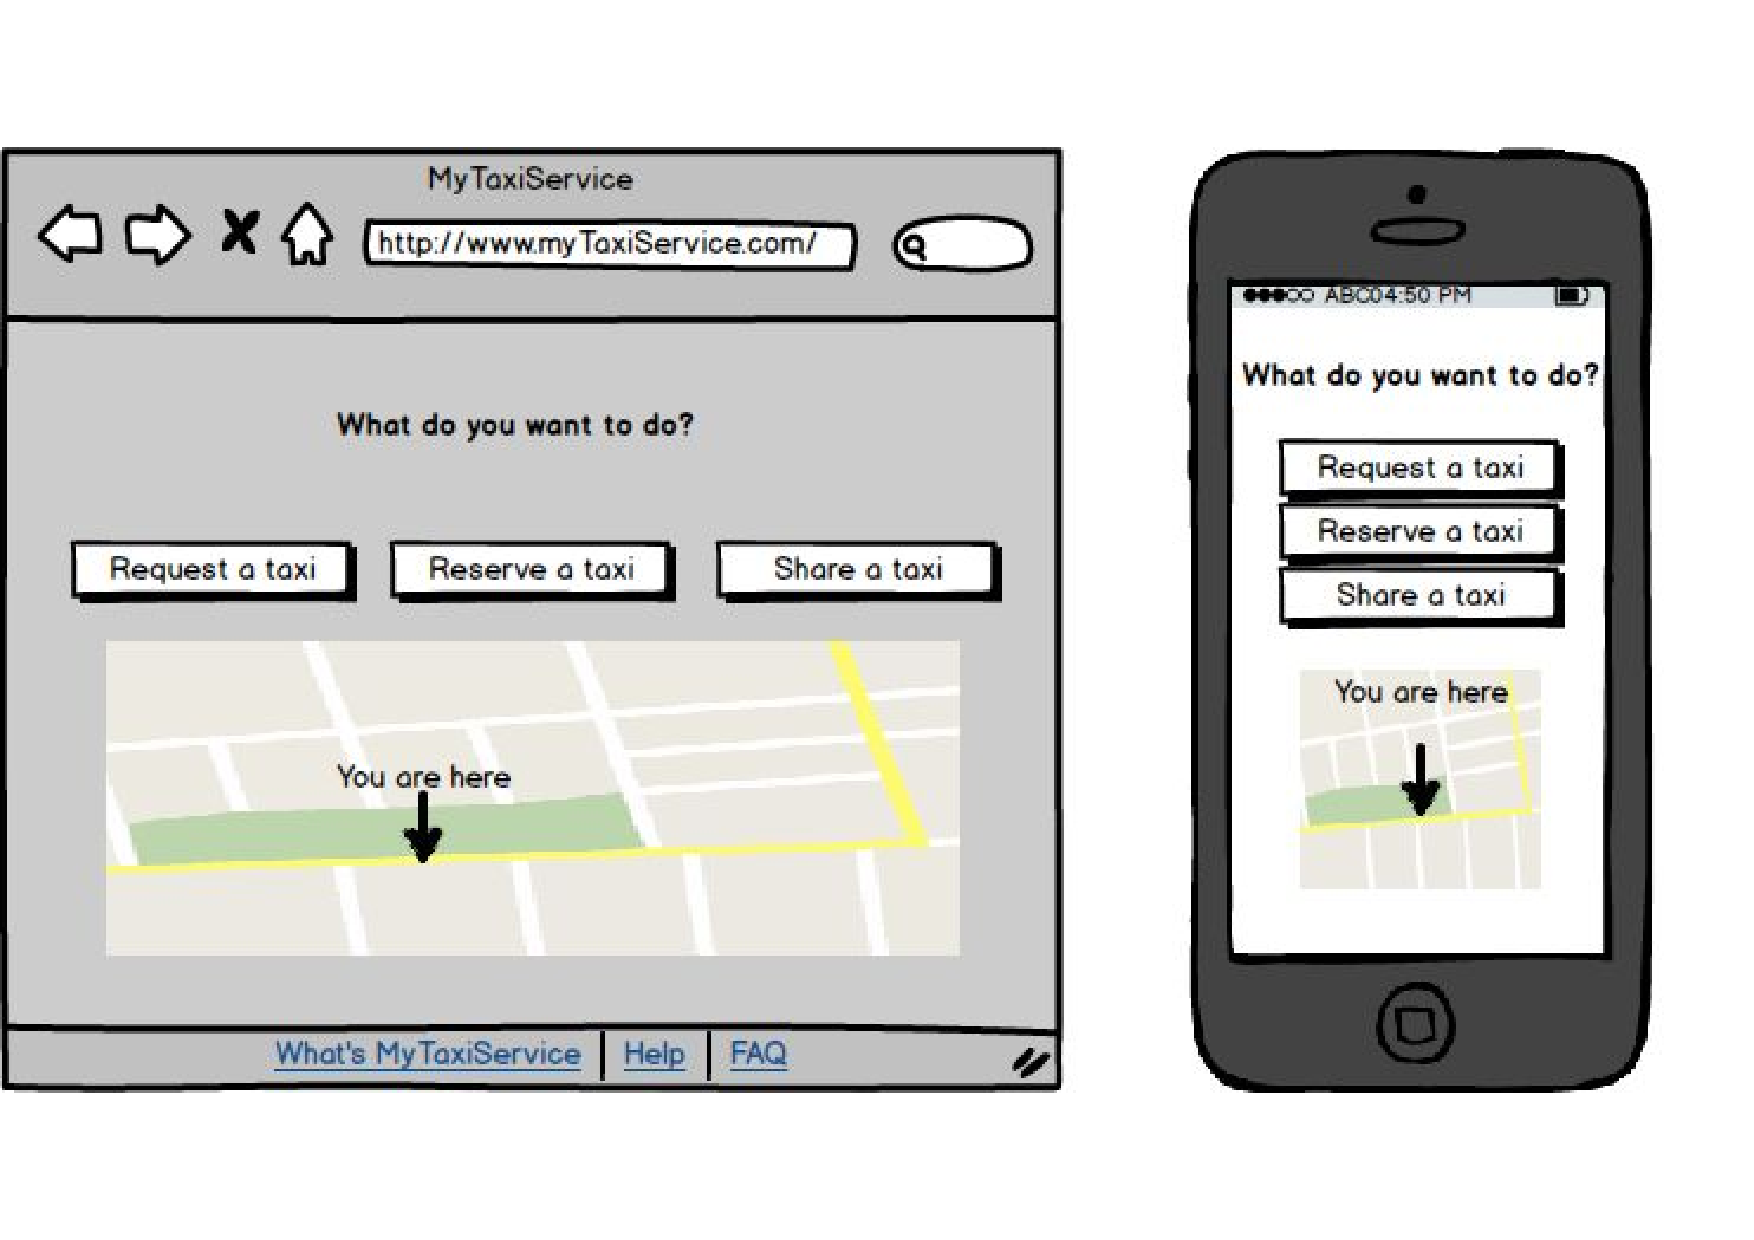
\includegraphics[width=\textwidth]{mockup/passengerFunctions.pdf}
\end{center}
\newpage
\paragraph{Request a taxi:}
View of the passenger when he/she requests a taxi
\begin{center}
	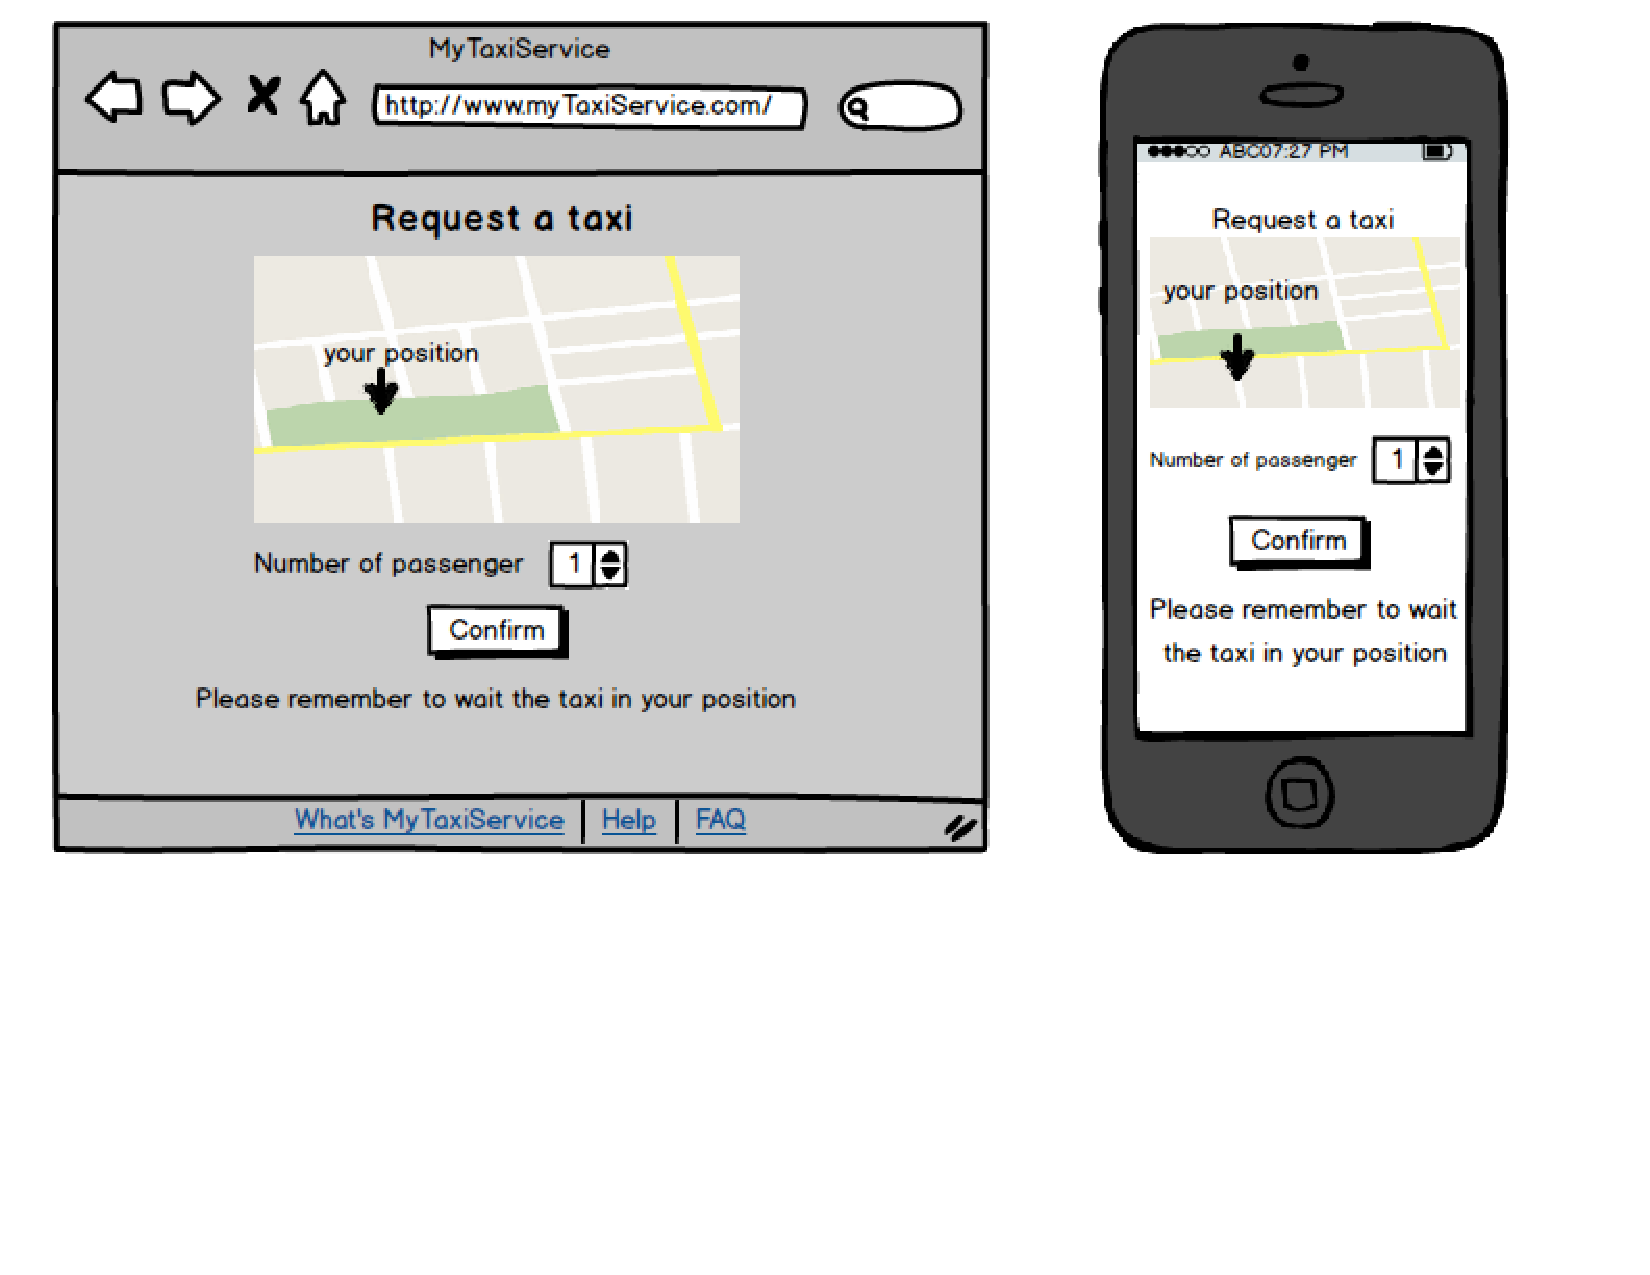
\includegraphics[width=\textwidth]{mockup/request.pdf}
\end{center}

\paragraph{Reserve a taxi:}
View of the passenger when he/she reserves a taxi
\begin{center}
	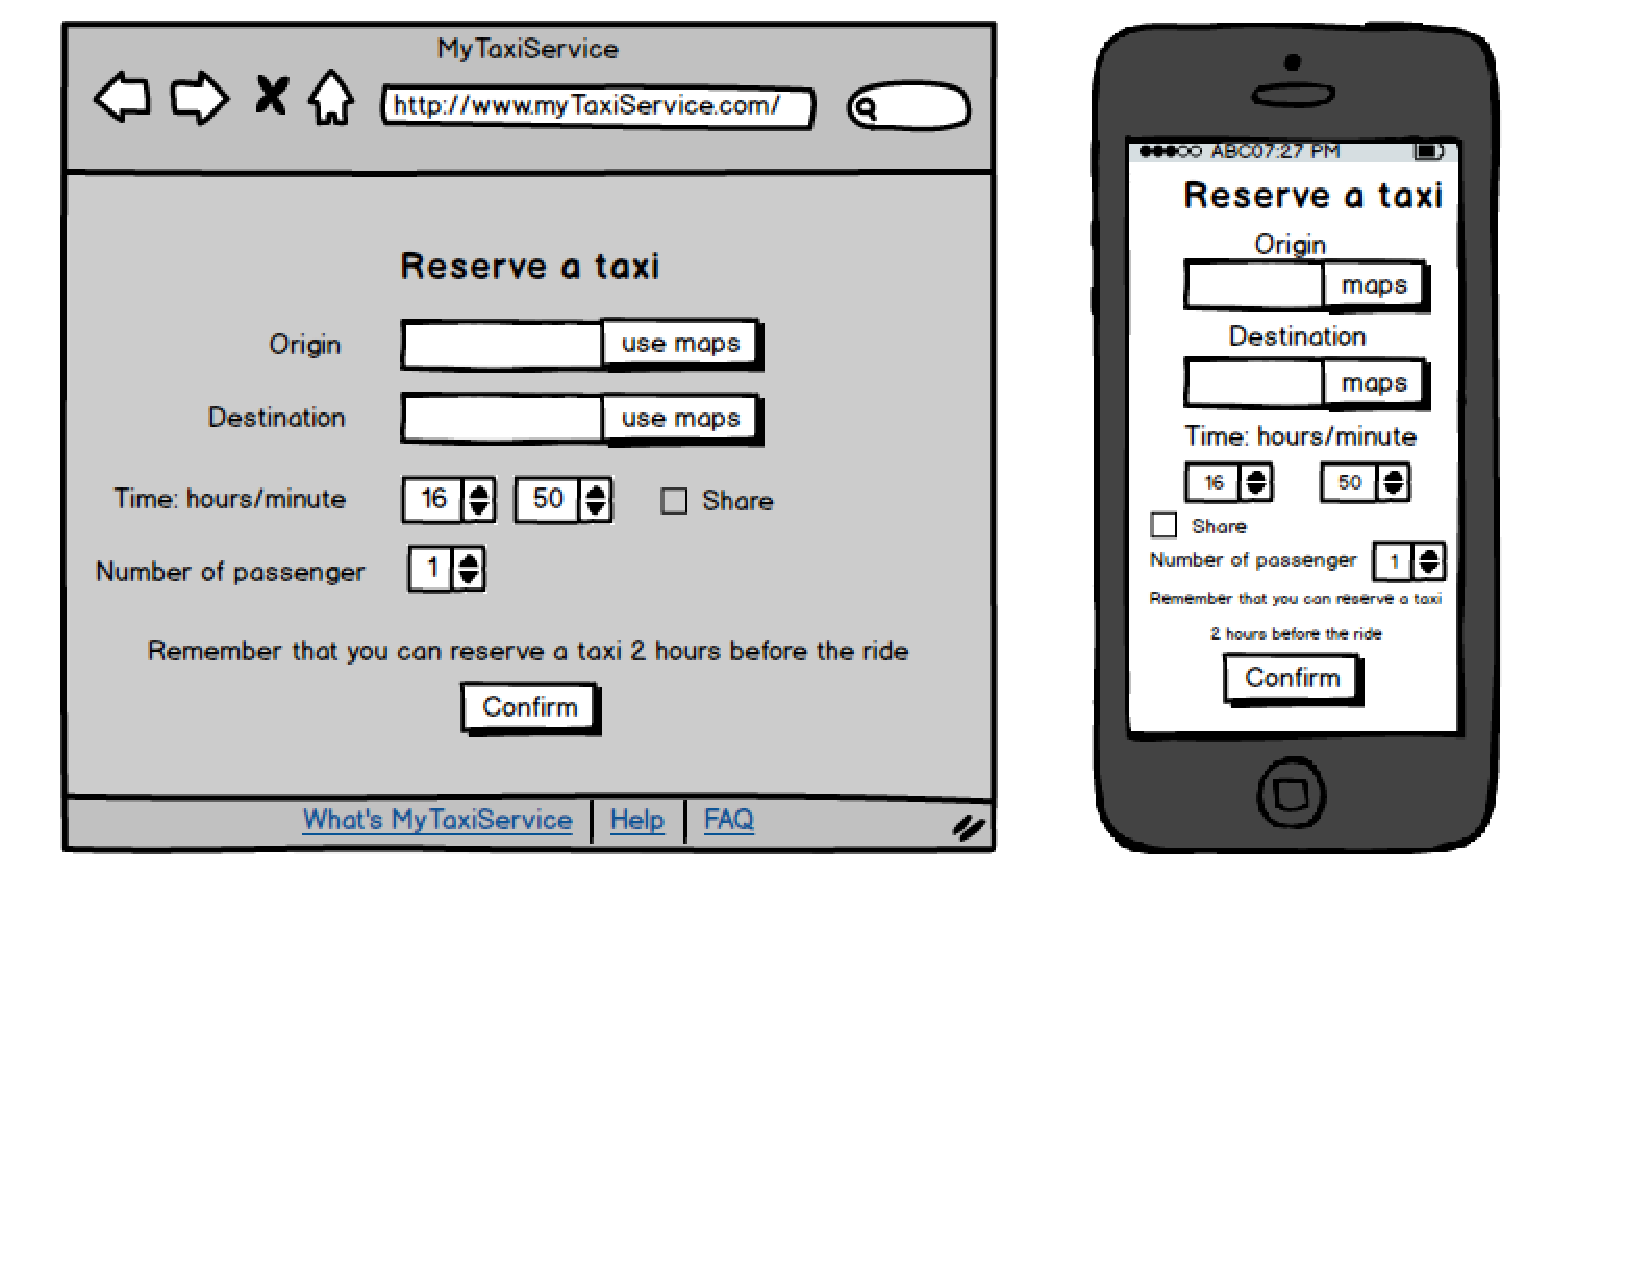
\includegraphics[width=\textwidth]{mockup/reserve.pdf}
\end{center}

\paragraph{Taxi driver view:}
View of the taxi driver
\begin{center}
	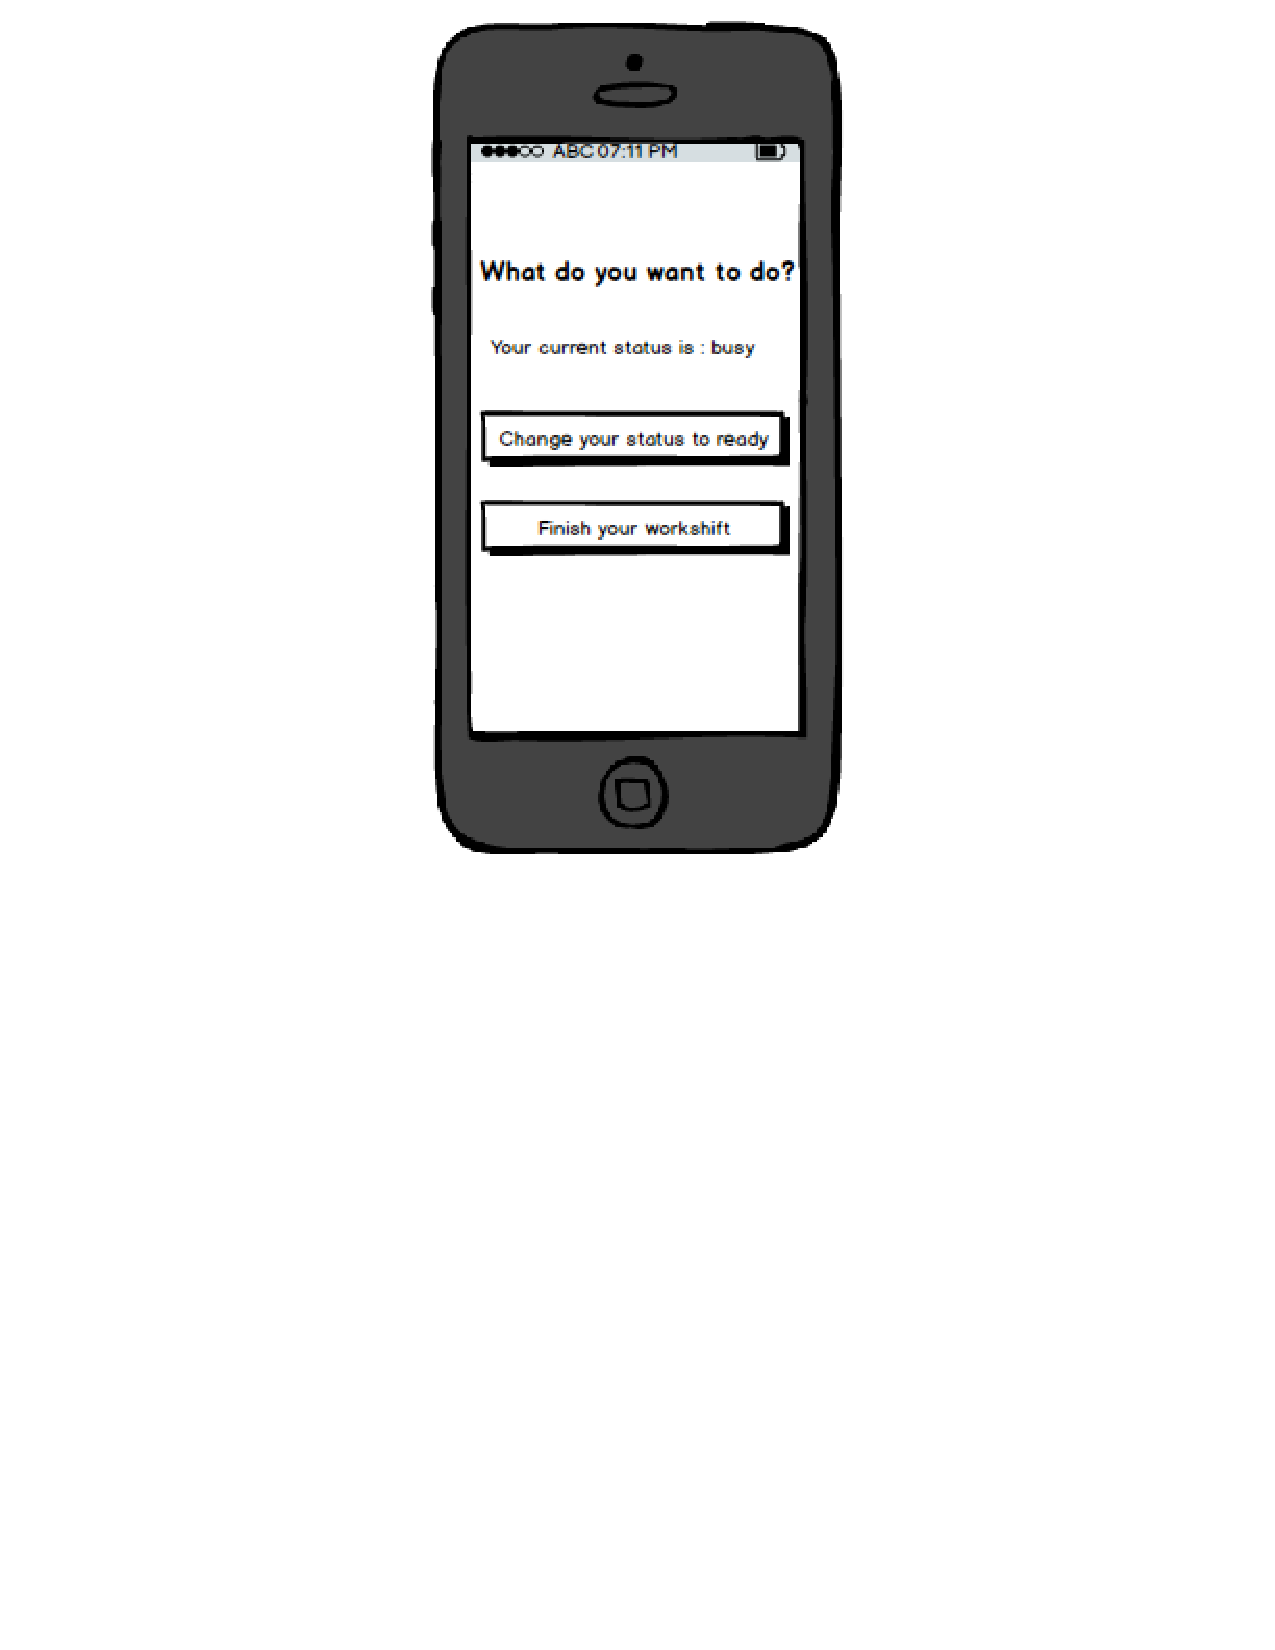
\includegraphics[width=\textwidth]{mockup/taxiDriverFunctions.pdf}
\end{center}
\newpage
\paragraph{Taxi driver notification:}
Notification that the taxi driver, choosen by the system, sees when a passenger request a ride.
\begin{center}
	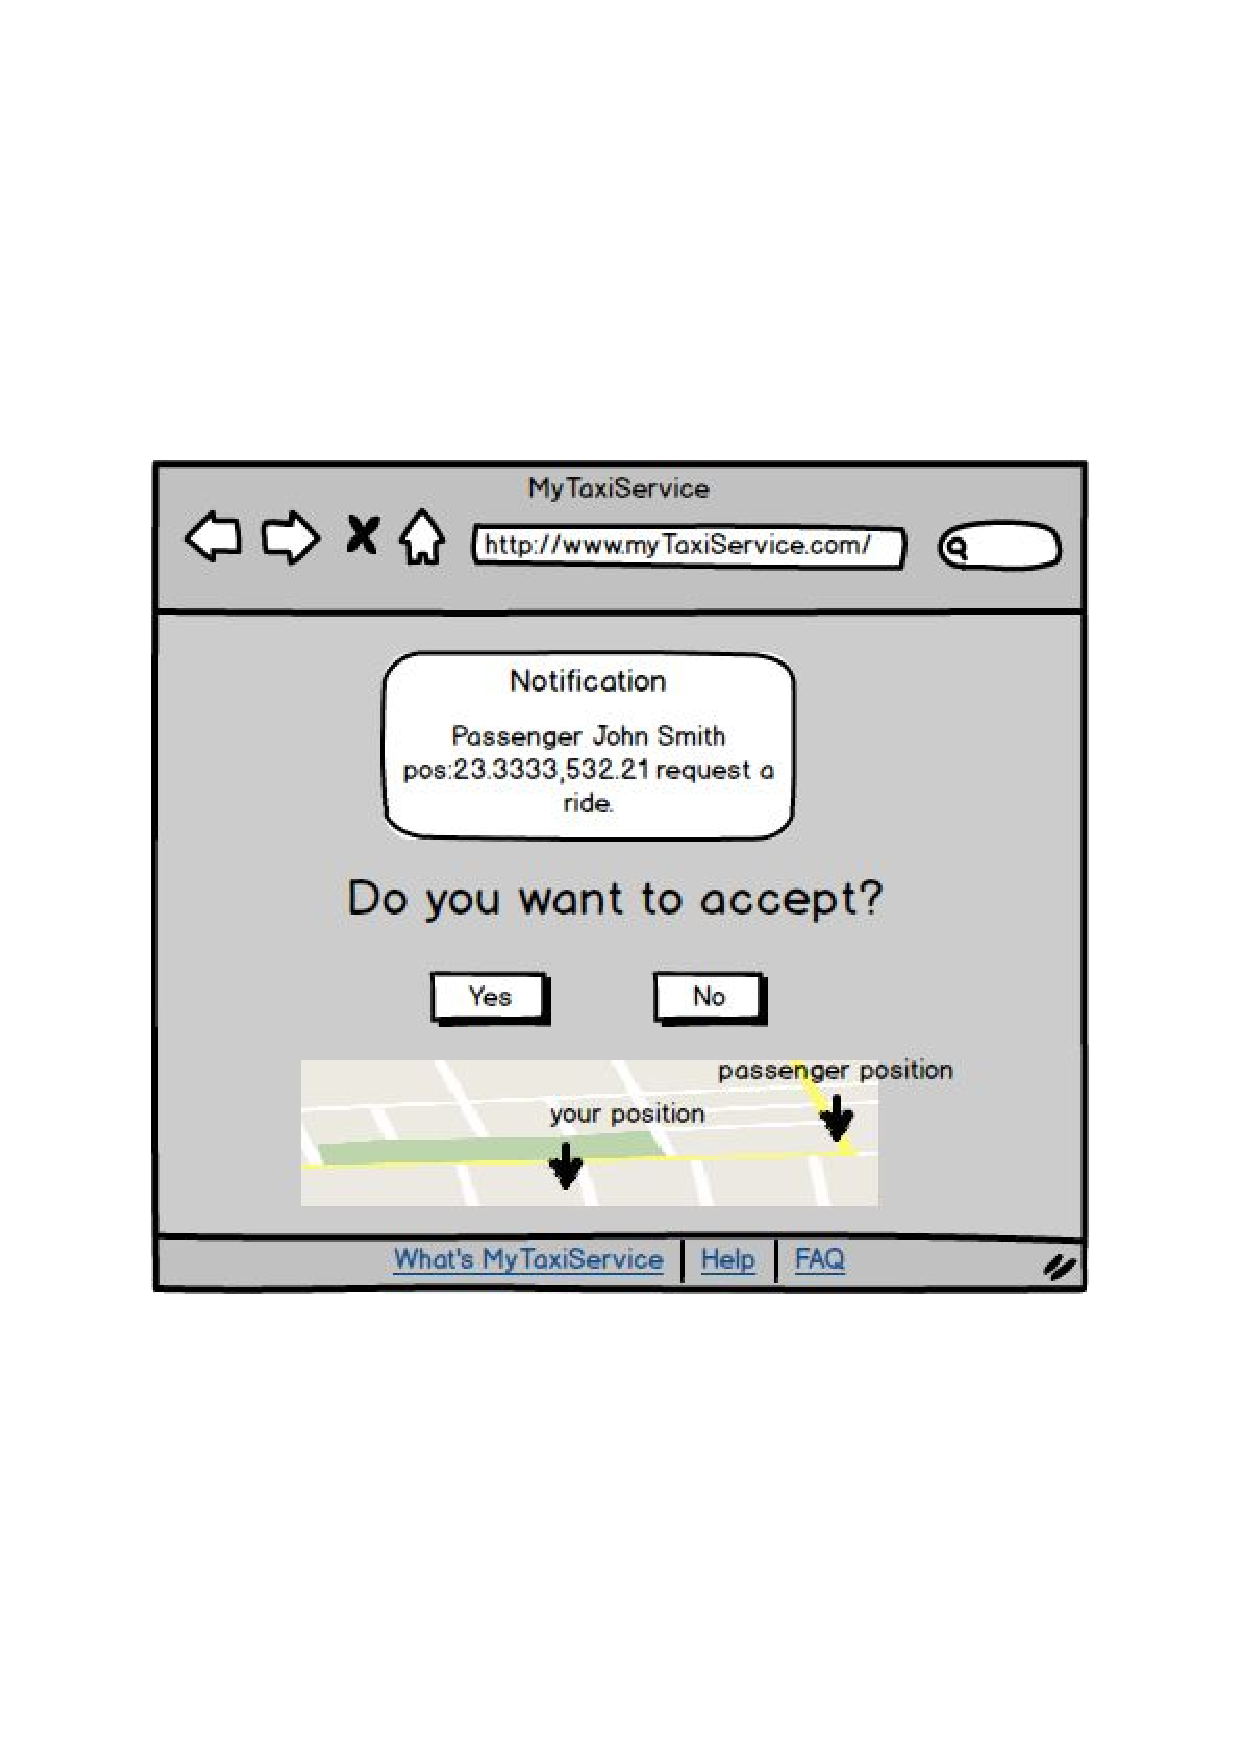
\includegraphics[width=\textwidth]{mockup/taxiDriverNotification.pdf}
\end{center}
\paragraph{Passenger notification :}
Notification that the passenger see when a taxi accept the ride
\begin{center}
	\includegraphics[width=\textwidth]{mockup/PassengerNotification.pdf}
\end{center}

\subsection{Hardware interfaces}
myTaxiService must have access to GPS of taxi driver's phones. GPS on passenger devices is not required.
\subsection{Software interfaces}
\begin{itemize}
	\item Database Management System (DBMS): \newline
	Name: MySQL \newline
	Version: 5.7 \newline
	Source: http://www.mysql.it/ 
	\item Java Virtual Machine (JVM):\newline
	Name: JEE \newline
	Version: 8 \newline
	Source: http://www.oracle.com/technetwork/java/javaee/tech/index.html
	\item Application server: \newline
	Name: Glassfish \newline
	Version: 4.1.1 \newline
	Source: https://glassfish.java.net/
	\item myTaxiService uses Google Maps APIs in order to show to the passengers and to the taxi driver their position in the city.
	This API is continuously update and works for all the OS and browsers web supported by myTaxiService.
	More information are available on the site: https://developers.google.com/maps/
\end{itemize}
\subsection{Communication interfaces}
\begin{itemize}
	\item Protocol: TCP Service: HTTPS Port : 443
	\item Protocol: TCP Service: HTTP  Port : 80
	\item Protocol: TCP Service: DBMS  Port : 9247
\end{itemize}


\section{Functional Requirements}
\subsection{Registration}
\paragraph{Purpose}
Visitors can register to myTaxiService through the web or mobile application. They can register either as a passenger or as a taxi driver.\\
In both cases, this operation requires the visitor to fill a registration form with personal data and accept myTaxiService terms and conditions, including personal data policies, according to local law. In case of registration as a taxi driver, the system requires the visitor more info, including proof of the possession of a valid taxi driver license.\\
If any of the previous requirements are not met or any input is invalid, the registration fails and the system asks the visitor to repeat the process. Otherwise, a verification email is sent to the provided email address: from that email the visitor can confirm his new account and successfully end the registration process.

\paragraph{Scenarios}
\begin{enumerate}
	\item Alex is a student. He has heard about myTaxiService and, finding it an easy way to travel, wants to subscribe to it.\\
	Therefore, he access to the homepage of the web application, clicks "Register", then chooses "Passenger". He fulfills the form, accepts the terms and conditions, and clicks "Confirm". However, the system cannot verify Alex's info because the confirmation password does not match with the first one. It therefore asks Alex to write it again. This time Alex fills the form correctly, then clicks "Confirm". The system verifies his info, then sends Alex a verification email to the submitted email address. Alex checks his mailbox, opens the new mail and clicks on the link inside it, redirecting him back to the web application of myTaxiService. The system informs him that the registration has successfully ended.
	He can now log in as a passenger user.
	
	\item Bob is a taxi driver. His company recommends him to subscribe to myTaxiService, in order to make his work easier and improve the taxi service.\\
	Therefore, he downloads and installs the mobile app of myTaxiService on his mobile phone, then opens it. He taps "Register", then chooses "Taxi Driver". He inputs all the required data, including his driver license ID, accepts the terms and conditions and confirms. The system verifies the submitted info and sends Bob a confirmation email. Bob checks his mailbox, opens the new mail and taps on the link inside. The system informs him that the registration has successfully ended. He can now log in as a taxi driver user.
\end{enumerate}

\paragraph{Diagrams}

\begin{center}
	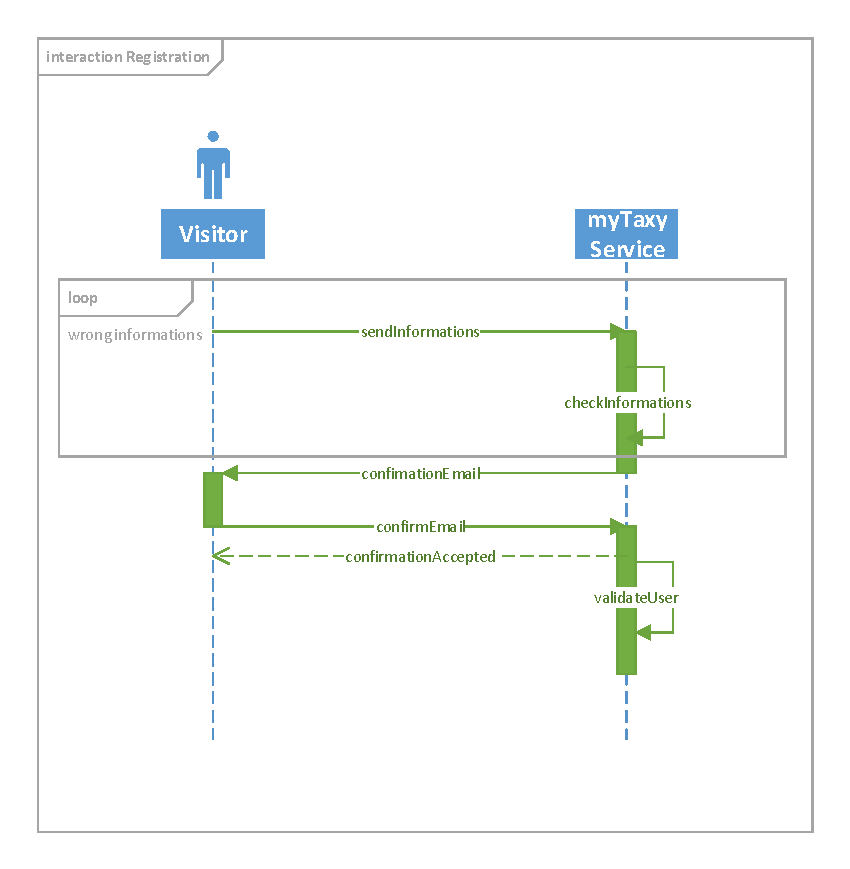
\includegraphics[height=\textwidth]{diagrams/registration}
\end{center}

\paragraph{Functional Requirements}
\begin{itemize}
	
	\item Visitors can register either as passengers or as taxi drivers.	
	\item Visitors can abort the registration process at any time.	
	\item The link in the confirmation email must be clicked within 1 day, otherwise the registration is deleted along with the visitor's info.	
	\item Registration forms contain the following info (fields):
	\begin{itemize}
		\item email address
		\item username
		\item password
		\item password confirmation
		\item name
		\item surname
		\item (*) address
		\item (*) telephone number
		\item (**) taxi license ID
		\item (**) taxi plate number
		\item (**) taxi code
	\end{itemize}
	All fields must be contain valid inputs.\\
	Fields marked with (*) are not mandatory.\\
	Fields marked with (**) are only for taxi driver registrations.	
	\item email address and username cannot be the same as ones from other myTaxiService users.	
	\item password must contain at least 8 characters.	
	\item password and password confirmation must match.	
\end{itemize}

\subsection{Login}

\paragraph{Purpose}
Visitors on myTaxiService website or mobile application may access to an existing registered user account providing its corresponding username (or email address) and password. In case the submitted info do not match with any existing account info, the system notifies the visitor that the username/email address doesn't exist, or that it exists, but the submitted password is wrong.\\
In case a user forgets his/her password, the system allows him/her to retrieve it, automatically creating a new password, setting it as the user's one and sending it to the provided email address.

\paragraph{Scenarios}
\begin{enumerate}
	\item Carl is a passenger user. He opens myTaxiService website, but can't remember his password to access the service. Therefore, he clicks on "Forgotten password?". The system asks him for the email address or username he provided at registration. He writes it down and clicks "Confirm". The system verifies the existence of the submitted email address, then creates a new password and sends it in an email to the submitted email address.
	
	\item Daisy is a passenger user, familiar with the myTaxiService website. She wants to use the mobile app, too. Knowing that she can enter either username or email and password, she fills both fields and clicks on "Log in". The system verifies her info: the operation ends successfully, and she gains access to the passenger user homepage.
\end{enumerate}

\paragraph{Diagrams}
\begin{center}
	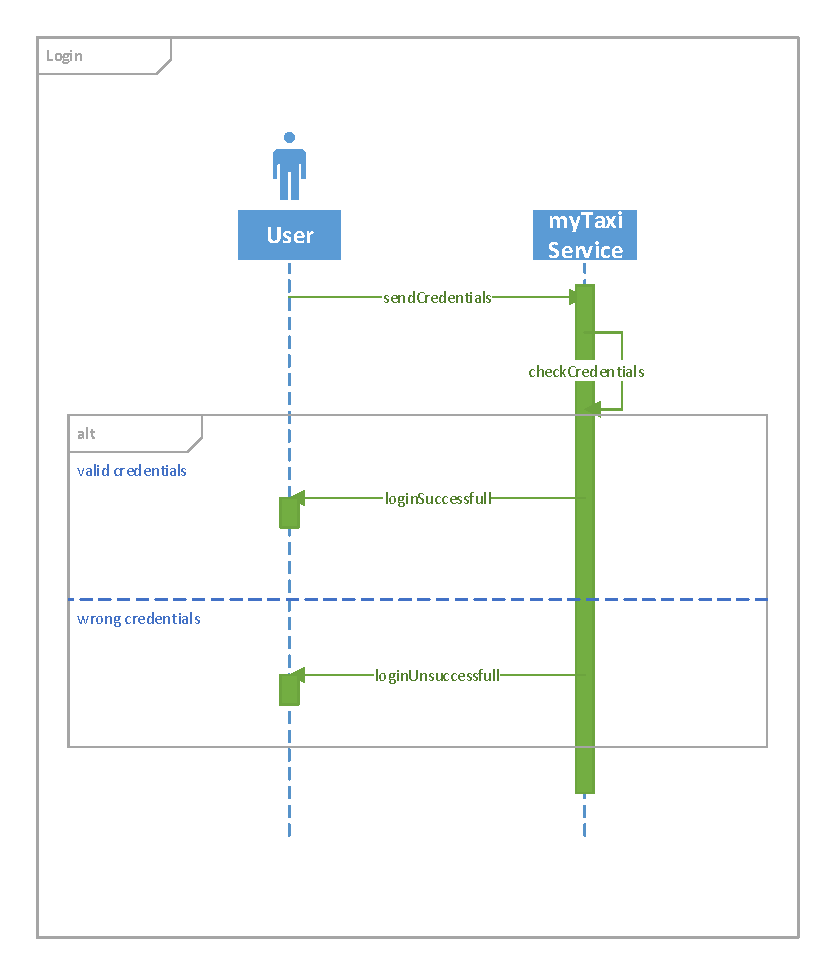
\includegraphics[height=\textwidth]{diagrams/login}
\end{center}
\paragraph{Functional Requirements}

\subsection{Standard ride request}

\paragraph{Purpose}

Passenger users can request a taxi both through the web or through the mobile application, giving only simple data about the number of passengers and sharing preferences (in case of shared ride, see also ?.?.?, "Shared Ride Request").\\
In any case, the system will then care about keeping the user informed about all details of his request, i.e. status of the request, estimated time of arrival (ETA) of the incoming taxi, in addition to its taxi code.

\paragraph{Scenarios}
\begin{enumerate}
	\item Elsa wanted to take the bus, but the heavy snow that fell in the last three days caused a lot of traffic problems. Fortunately for her, the taxi service is still functioning, so she opens myTaxiService on her mobile phone, logs in, and chooses "Request".
	She uses the GPS info to fill the "Origin" field, leaves the "Share" checkbox blank, then "Confirm". In a matter of minutes Frank, a taxi driver in her zone, accepts her request: Elsa is informed that she has to wait approximately 6 minutes for her taxi, encoded 288, to arrive. In the meanwhile, the system give her updates about the taxi position. At the expected time Frank arrives, picks Elsa up and carries her to desired destination.
\end{enumerate}

\paragraph{Diagrams}

\paragraph{Functional Requirements}
\begin{itemize}
	
	\item The system allows taxi ride requests if and only if the passenger accepts to give info about his/her location, either through GPS or directly writing down a valid location.
	
	\item The system allows taxi ride requests if and only if the passenger can be located in some definite position of some definite taxi zone.
	
	\item The system uses default values for the number of passengers and sharing preferences of a ride (1 person, no sharing), unless the passenger does specify them.
	
	\item The system uses a FIFO policy to manage forwarding of pending ride requests.
	
	\item The system uses a FIFO policy to manage the order of taxi drivers in queues to send notifications to.
	
	\item The system forwards a ride request to the first taxi driver in the considered zone queue if and only if he/she has a sufficient number of free seats available in his/her vehicle.
	
	\item The system keeps the passenger(s) notified about the status of the ride request he/she sent.
	
	\item Once a ride request has been accepted by some taxi driver, the system changes the request status from "Pending" to "Accepted".
	
	\item Once a ride request has been accepted by some taxi driver, the system calculates the ETA of the incoming taxi based on the distance between the taxi and the passenger(s), and the current traffic.
	
	\item Once a ride request has been accepted by some taxi driver, the system notifies the passenger(s) about the ETA of the incoming taxi.
	
	\item Once a ride request has been accepted by some taxi driver, the system keeps the passenger(s) notified about the current location of the incoming taxi, showing its position on a map.
	
	\item Once a ride request has been accepted by some taxi driver, the system prevents the passenger(s) to make a new ride request until the taxi driver changes the status of the ride to "Completed".
\end{itemize}

\subsection{Reserved ride request}

\paragraph{Purpose}
Passenger users can request to reserve a taxi for some definite future ride. The operation can be done both through the web or through the mobile application, and requires information about the location and exact date and time of the meeting point, the destination, the number of passengers and the sharing preferences (in case of shared ride, see also ?.?.?, "Shared Ride Request").\\
In any case, the system will then care about sending a taxi to the given location at the given date and time. Reservation requests must occur at least two hours before the ride meeting time.

\paragraph{Scenarios}
\begin{enumerate}
	\item George has an important meeting tomorrow morning, but his car suddenly broke. He decides he will take a taxi. Therefore, he opens the homepage of myTaxiService web application on his laptop, logs in as a passenger user, then clicks "Reserve". He selects "use maps" for both position fields, and pinpoints his home and the location of the meeting as "Origin" and "Destination", respectively. He selects "7.15" as the meeting time, leaves the "Share" checkbox blank, then clicks "Confirm".\\
	The next day, at 7.05, a reserved ride requests is received by Harry, the first taxi driver in the queue of the taxi zone where George's meeting point is located. Harry decides to refuse the request, though. The request is then forwarded to Isabelle, which was the second taxi driver in queue at the time of Harry's refusal. She accepts George's request, and at the given time arrives at his house. She picks him up and brings him to the meeting.
\end{enumerate}

\paragraph{Diagrams}

\paragraph{Functional Requirements}

\subsection{Shared ride request}

\paragraph{Purpose}

\paragraph{Scenarios}

\paragraph{Diagrams}

\paragraph{Functional Requirements}

\subsection{Request notification and response}

\paragraph{Purpose}

\paragraph{Scenarios}

\paragraph{Diagrams}

\paragraph{Functional Requirements}

\subsection{Availability settings}

\paragraph{Purpose}
Taxi drivers are able to notify the system about their status through the mobile application at any moment, as long as they're logged in. In particular, the status can be either "Ready", "Busy" or "Offline".\\
Whenever a taxi driver logs in, the system automatically sets his/her status from "Offline" to "Ready" and put him/her on the bottom of its current taxi zone queue, based on GPS info.\\
When he/she accepts a taxi ride, the status is automatically updated to "Busy": the system then removes him/her from the queue, preventing the arrival of other ride requests.\\
Similarly, when the ride is over, the taxi driver has to notify the system that the ride has ended: the system automatically changes the status back to "Ready" and puts him/her back on the bottom of the current taxi zone queue, thus waiting for a new ride request.\\
Finally, when the taxi driver finishes his workshift, he may inform the system, or simply log off. In both cases, his/her status automatically switches to "Offline".

\paragraph{Scenarios}
Albert is a taxi driver subscribed to myTaxiService. He logs in through his mobile phone and his status changes from "Offline" to "Ready". The system receives info from the GPS and puts Albert on the bottom of the taxi zone he's currently in. After a while, his phone notifies him about a new ride request: he decides to accept it and his status changes to "Busy". He's no longer in the taxi queue. Albert goes to the start location, picks up Barbara and takes her to her destination. When they arrive, Albert informs the system that he has concluded the ride: his status changes to "Ready". The system puts him on the bottom of his current taxi zone queue. Later on, he receives another ride requests, but this time he decides to refuse it: its status remains unchanged as "Ready", but he loses all his positions in the queue.
A few hours later, Albert finishes his worktime and logs off. The system sets his status to "Offline" and removes him from any queue.

\paragraph{Diagrams}

\paragraph{Functional Requirements}
\begin{itemize}
	
	\item The system uses a FIFO policy to manage taxi zone queues.
	
	\item The system uses info provided by the GPS to locate taxis and decide their respective queues.
	
	\item The system automatically inserts taxi drivers in queues when their status changes to "Ready".
	
	\item The system automatically removes taxi drivers from queues when their status changes to "Busy" or "Offline".
	
	\item The status automatically changes to "Busy" when the taxi driver accepts a ride request.
	
	\item The status automatically changes to "Ready" when the taxi driver notifies the end of a ride.
	
	\item When status is "Ready", the application notifies about ride requests.
	
	\item When status is "Ready", the application enables the taxi driver to accept/refuse requests.
	
	\item When status is "Busy", the application prevents ride requests notifications.
	
	\item When status is "Busy", the application enables the taxi driver to notify the end of the current ride.
	
\end{itemize}

\subsection{Account Settings}

\paragraph{Purpose}
The system allows registered users to view and modify their profiles at any moment, as long as they're logged in. Usernames cannot be modified, while modified email addresses, taxi license IDs and taxi codes must not match with the ones of other users, otherwise the system denies the modification request. In case of modified email address, the system sends a confirmation email to the new address. Modification will succesfully ends when the user clicks the link in the sent email. 

\paragraph{Scenarios}
Alex uses to periodically change his account password, in order to increase protection. To do so, every 3 months, he opens myTaxiService on his mobile phone, chooses "Profile", then "Modify". He selects the password field, writes down a new one, then writes it again in the "Confirm password" field. Finally, he clicks "Confirm": the system informs him that his account password has succesfully been updated.

\paragraph{Diagrams}

\paragraph{Functional Requirements}


\section{The world and the machine}
\input{specific_requirements/the_world.tex}

\section{Scenarios}
\input{specific_requirements/scenarios.tex}

\section{UML Models}
\input{specific_requirements/uml_models.tex}

\section{Non Functional Requirements}
\section{Performance Requirements}
%TODO
myTaxiService will perform 95\% of the operations within 4 seconds; the total amount of the operations within 10 seconds.
The system should ensure at least 2000 passangers connected and 500 taxi drivers connected.

\section{Design constraints}
myTaxiService wants to reach most of taxi drivers and passengers, requiring minimum specifications for devices.
Taxi drivers, registered to the system, have to use their own devices provided with GPS navigation system to perform the service. Mobile applications have to offer backward compatibility.

\section{Software system attributes}
\paragraph{Reliability}
The mean time between failures (MTBF) shall exceed 3 months.
\paragraph{Availability}
In order to maintain the system up-to-date and secure, myTaxiServer schedules downtime periods where will be executed routine operations. The service should be available 99\% of the time.
\paragraph{Security}
myTaxiService to ensure service availability and data protection use:
\begin{itemize}
	\item AES cryptography algorithm on network operations
	\item Data are encrypted and stored in backup drives to prevent system failure
	\item Login authentication. Users, after the registration, have to confirm their e-mail with the security code sent to the e-mail write in the registration form
	\item SQL injection detection
\end{itemize}
Server architecture will be implemented separating
data from application. Application server must be separated
from database and from the web server. All architectures are divided by firewalls.
\paragraph{Maintainability}
To ensure an easy maintenance of the software, it must be well-documented and written following coding patterns.
\paragraph{Portability}
Web programming ensures a wide target of browser. Mobile applications instead, cause of different languages and devices, have to be written following coding patterns for easy portability.
Availability of the service is ensured by hardware and software limitations in Section 2.4.2.



%\chapter{Appendix}
%
%\section{Alloy}
%
%\section{Software and tool used}
%
%\section{Hours of works}
%
%\chapter{Revision}
%
%\section{Changed Assumptions}
%
%\section{Removed goal and functionality}
%
%\section{Modified Functional Requirements}
%
%\section{Modified scenarios and Use Cases}
%
%\section{Modified Diagrams}
\end{document}
       
